\documentclass[12pt]{article}
\usepackage[letterpaper, margin=1in]{geometry}
\usepackage{graphicx}
\usepackage{xfrac}
\usepackage{anyfontsize}
\usepackage{verbatim}
\usepackage[framed, numbered]{matlab-prettifier}
\lstset{inputpath=../Matlab}
\graphicspath{{../Figures/}}
\title{ELECENG 3TP3 Lab 1}
\author{Raeed Hassan \\ hassam41 \\ McMaster University}
\begin{document}
\maketitle
\pagebreak
\section*{Question 1}
To plot the discrete time signals listed, it was first necessary to create functions for the unit step function, $u[n]$, and the unit impulse function, $\delta[n]$. The MATLAB code for the unit step function is shown in Listing \ref{listing:unitstep}, and the Matlab code for the unit impulse function is shown in Listing \ref{listing:unitimpulse}.
\lstinputlisting[style=Matlab-editor, caption={unit step function}, label={listing:unitstep}]{unitstep.m}
\lstinputlisting[style=Matlab-editor, caption={unit impulse function}, label={listing:unitimpulse}]{unitimpulse.m}
Once the unit step and unit impulse functions have been defined in their own .m files, we can use these to define the specified discrete time signals. We can simply add the individual terms of each signal to calculate the resulting discrete time signal. The Matlab code to calculate each discrete time signal is shown in Listing \ref{listing:question1_signals}.
\lstinputlisting[style=Matlab-editor, caption={Question 1 Signals}, label={listing:question1_signals}, firstline=1, lastline=6]{question1.m}
The defined discrete time signals can be plotted in MATLAB using the stem function. The MATLAB code used to plot these graphs and create an image of the figure generated is shown in Listing \ref{listing:question1_plots}, and the image of the plots is shown in \ref{fig:question1_plots}. 
\lstinputlisting[style=Matlab-editor, caption={Question 1 Plotting the Signals}, label={listing:question1_plots},firstnumber=8,firstline=8,lastline=26]{question1.m}
\begin{figure}[!ht]
    \centering
    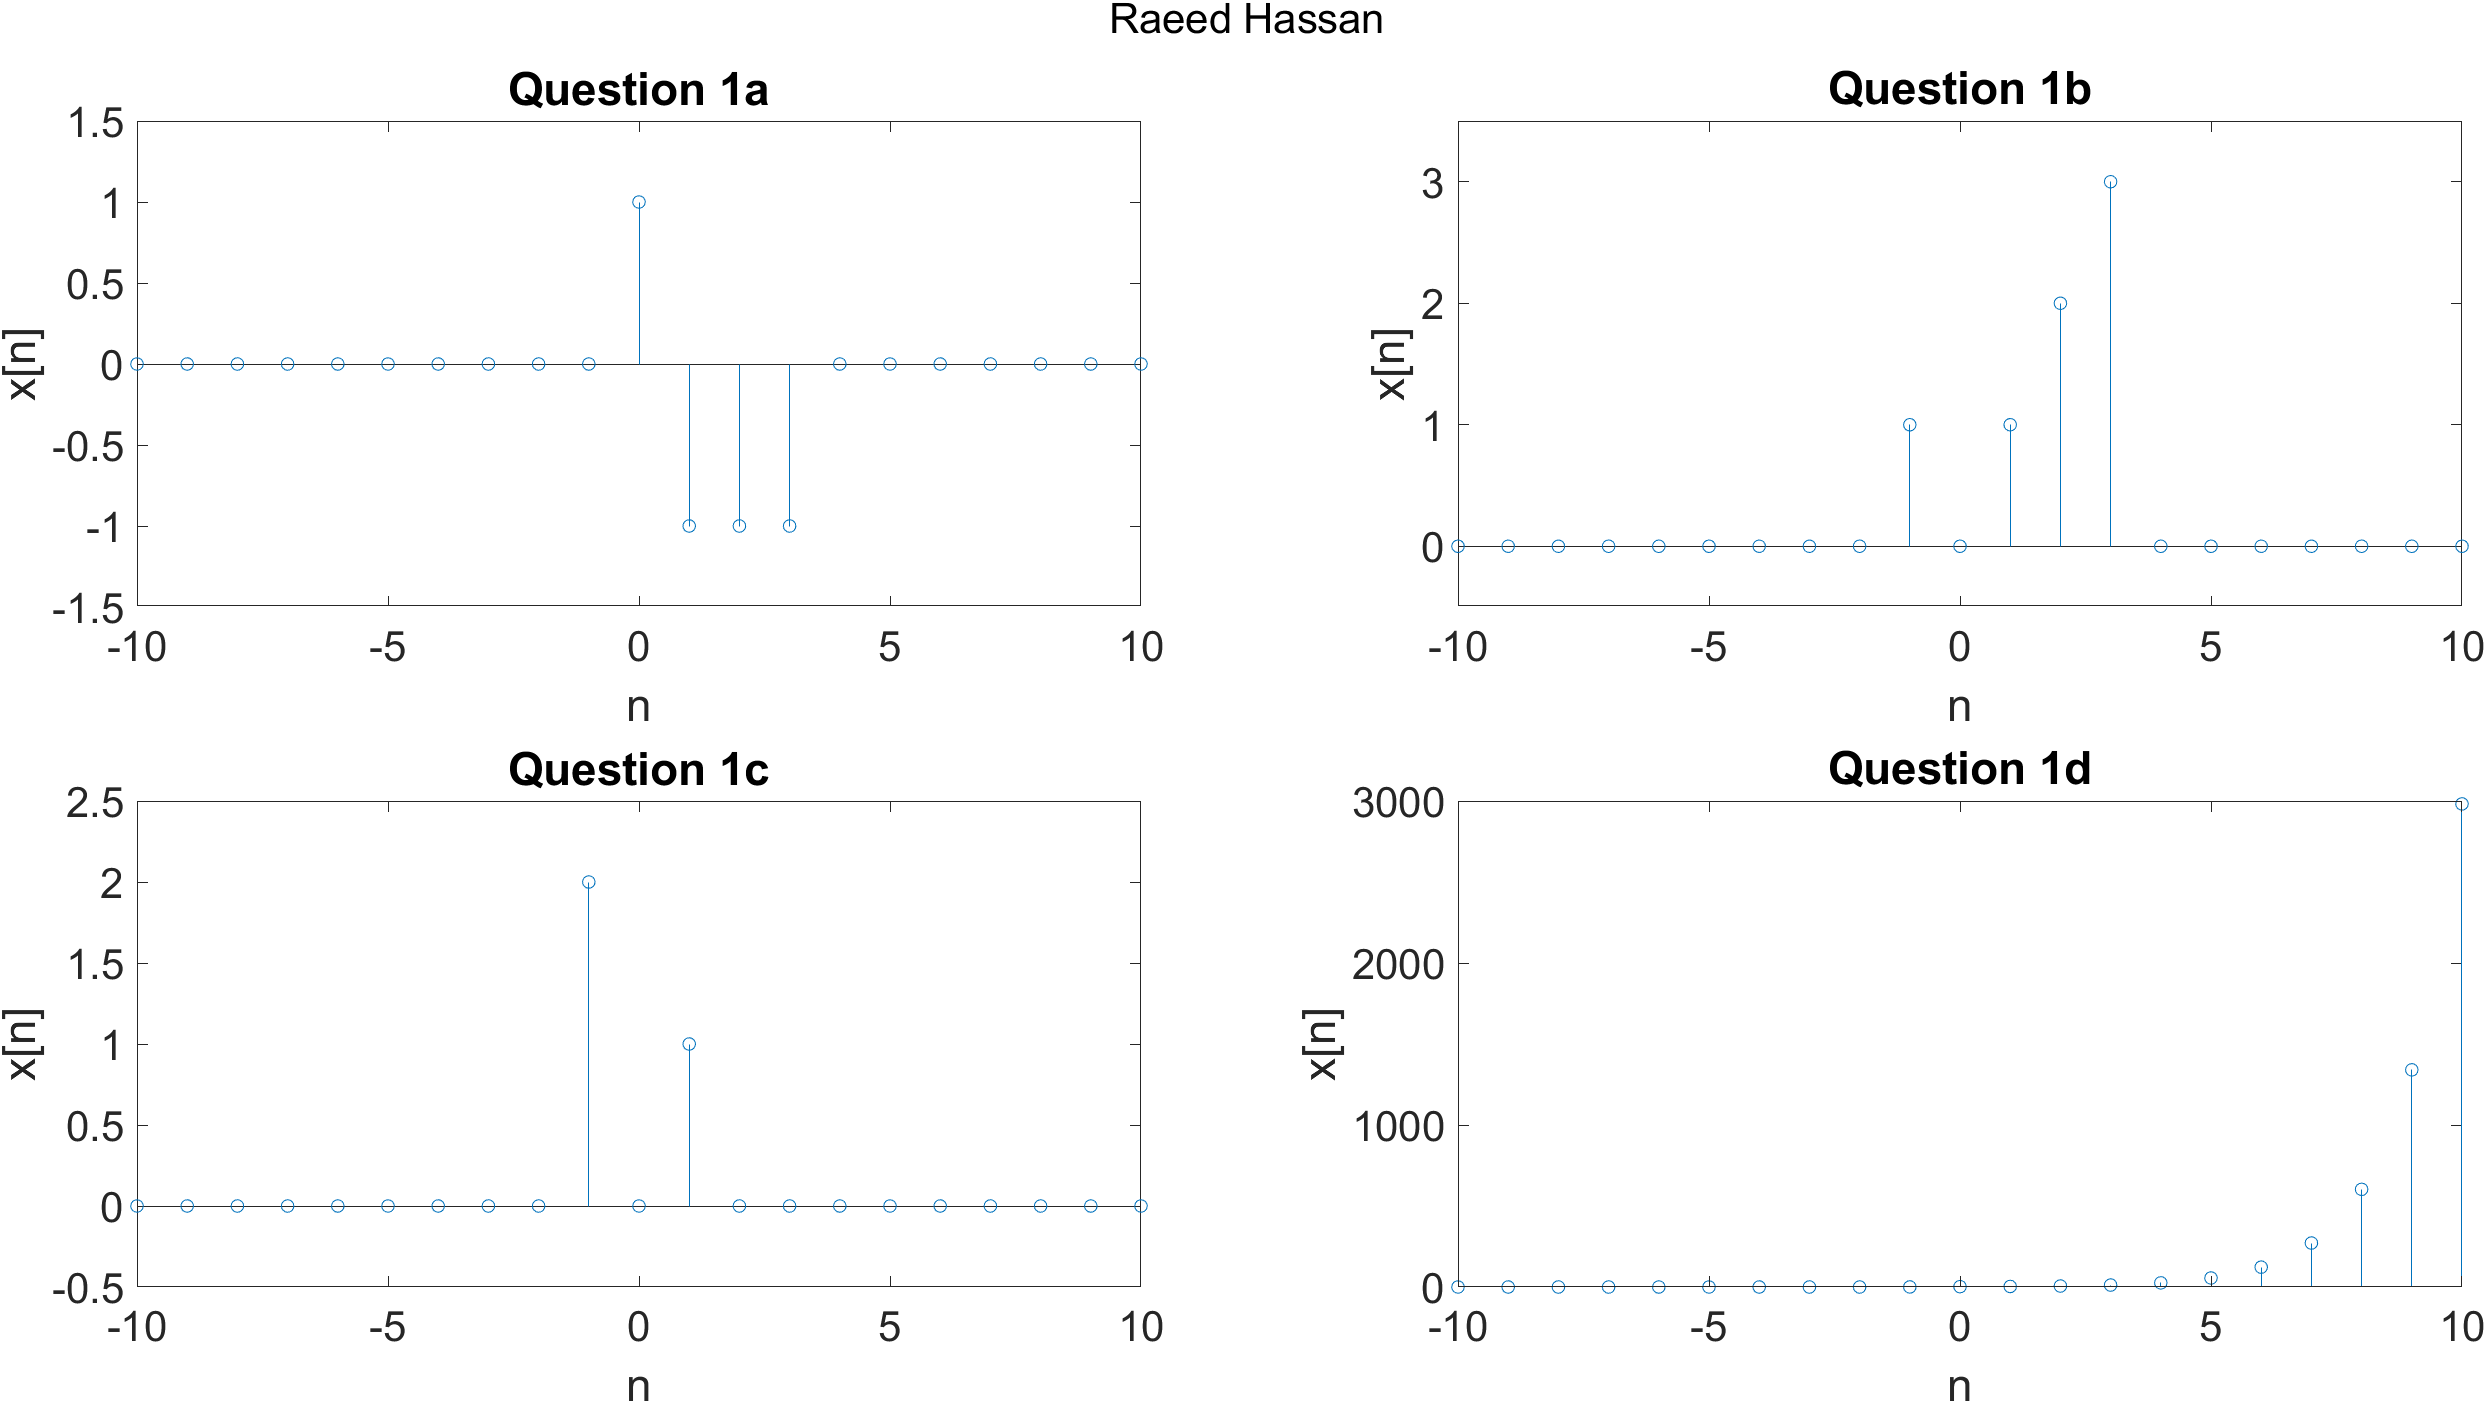
\includegraphics[width=0.85\textwidth]{question1.png}
    \caption{Question 1 Plots}
    \label{fig:question1_plots}
\end{figure}
\pagebreak
\section*{Question 2}
\subsection*{2a}
The MATLAB function, named question2a, accepts three inputs: the set of student grade records as a matrix, the maximum grade vector, and a vector of column indices. The function performs element-wise division on every grade in the student grade records matrix, grades, by their maximum value in the maximum grade vector, maximum. The resulting matrix contains every grade relative to its maximum grade (a grade of 1). The sum of each row is calculated using Matlab's sum function, then divided by the number of columns to determine the average grade for each student. Every element in the vector is multiplied by 100 to convert the grades to a percentage. The Matlab code for the function is shown in Listing \ref{listing:question2a}.
\lstinputlisting[style=Matlab-editor, caption={Question 2a}, label={listing:question2a}]{question2a.m}
\subsection*{2b}
The input for the function created in 2a requires a matrix of the student grace records and a vector of the maximum grades, which were created by using MATLAB's csvread function on the appropriate rows and columns of the course\_grades\_2020.csv file and stored in \verb|student_grades| and \verb|max_grades|. The columns for lab grades and exam grades were defined in \verb|lab_columns| and \verb|exam_columns|. These were used as inputs for the function created in 2a to calculate average lab and exam marks for each student, stored in the vectors \verb|lab_averages| and \verb|exam_averages|. The overall course averages for labs and exams were calculated by using Matlab's mean function on the vectors. The Matlab code for question 2b is shown in Listing \ref{listing:question2b}.
\lstinputlisting[style=Matlab-editor, caption={Question 2b}, label={listing:question2b},lastline=16]{question2b.m}
\subsection*{2c}
The MATLAB script for question 2c is similar to the script used in 2b. In addition to the code used to calculate the student averages for the labs and exams, it uses the column for the midterm grades, \verb|midterm_column|, to calculate the student averages for the midterm, stored in the vector \verb|midterm_averages|. The weighted average of the lab, midterm, and exam average vectors is calculated and stored in the vector \verb|final_grades|. To create a plot of the final grades in decreasing order, the final grades are sorted using Matlab's sort function, then plotted using Matlab's bar function. The Matlab code for question 2c is shown in Listing \ref{listing:question2c}. The plot of the final grades in decreasing order of final grade is shown in Figure \ref{fig:question2c}. 
\lstinputlisting[style=Matlab-editor, caption={Question 2c}, label={listing:question2c}]{question2c.m}
\begin{figure}[!ht]
    \centering
    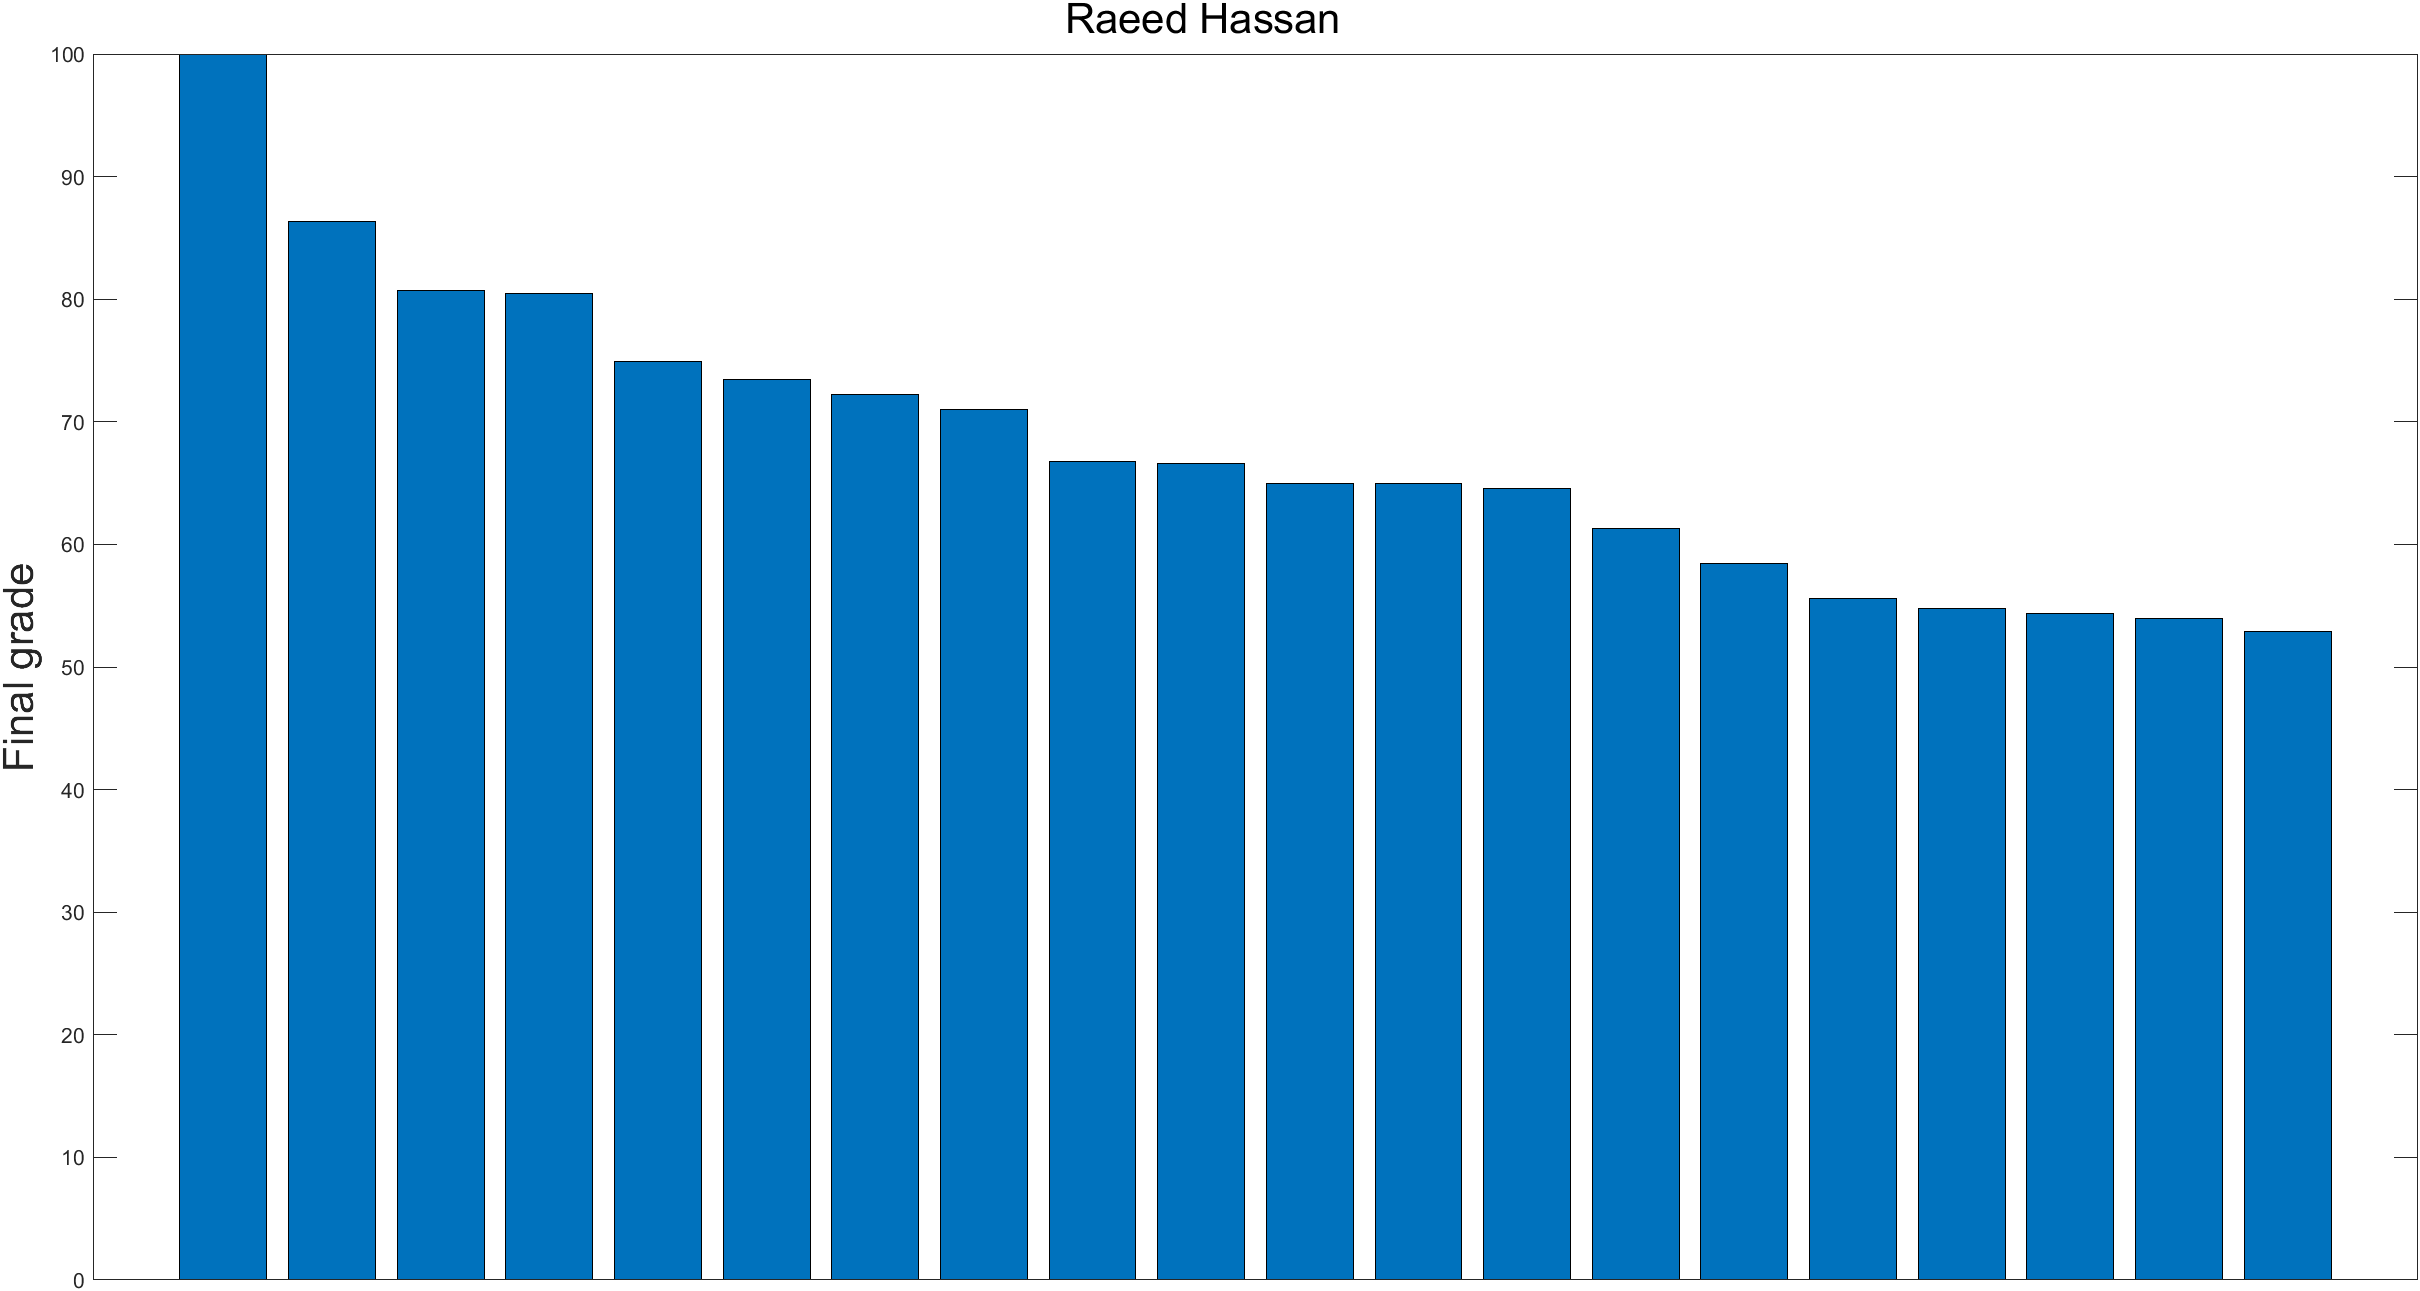
\includegraphics[width=\textwidth]{question2c.png}
    \caption{Question 2c}
    \label{fig:question2c}
\end{figure}
\pagebreak
\section*{Question 3}
\subsection*{3a}
A visualization of the greyscale integer values is done in 3a, showing the range of the greyscale integer values of the ee3top3picture2020.png image. From this data, we can see that the values are very condensed and take up only a small portion of the entire greyscale range (0 to 255). Upon closer inspection, we can find that the minimum and maximum values of the image are 159 and 187, occupying only 29 of the possible 256 values.
\lstinputlisting[style=Matlab-editor, caption={Question 3a}, label={listing:question3a},firstnumber=3,firstline=3,lastline=11]{question3.m}
\begin{figure}[!ht]
    \centering
    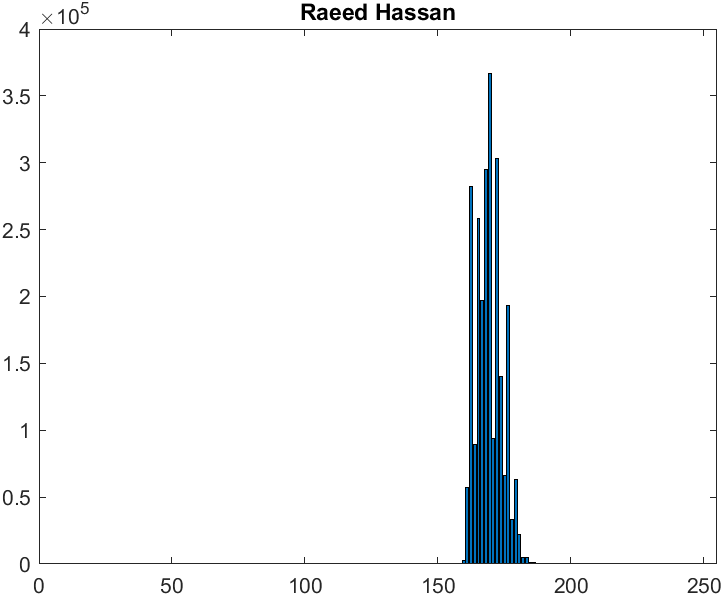
\includegraphics[width=0.81\textwidth]{question3a.png}
    \caption{Question 3a}
    \label{fig:question3a}
\end{figure} \pagebreak
\subsection*{3b}
The MATLAB code for displaying and printing the image is shown in Listing \ref{listing:question3b}. The image exported by MATLAB is shown in Figure \ref{fig:question3b}. The image has very poor contrast, likely due to the limited range of greyscale values that was determined in 3a. It is difficult to dintiguish parts of the image because their greyscale values are very close, resulting in the image have very little difference in colour or darkness.
\lstinputlisting[style=Matlab-editor, caption={Question 3b}, label={listing:question3b},firstnumber=13,firstline=13,lastline=16]{question3.m}
\begin{figure}[!ht]
    \centering
    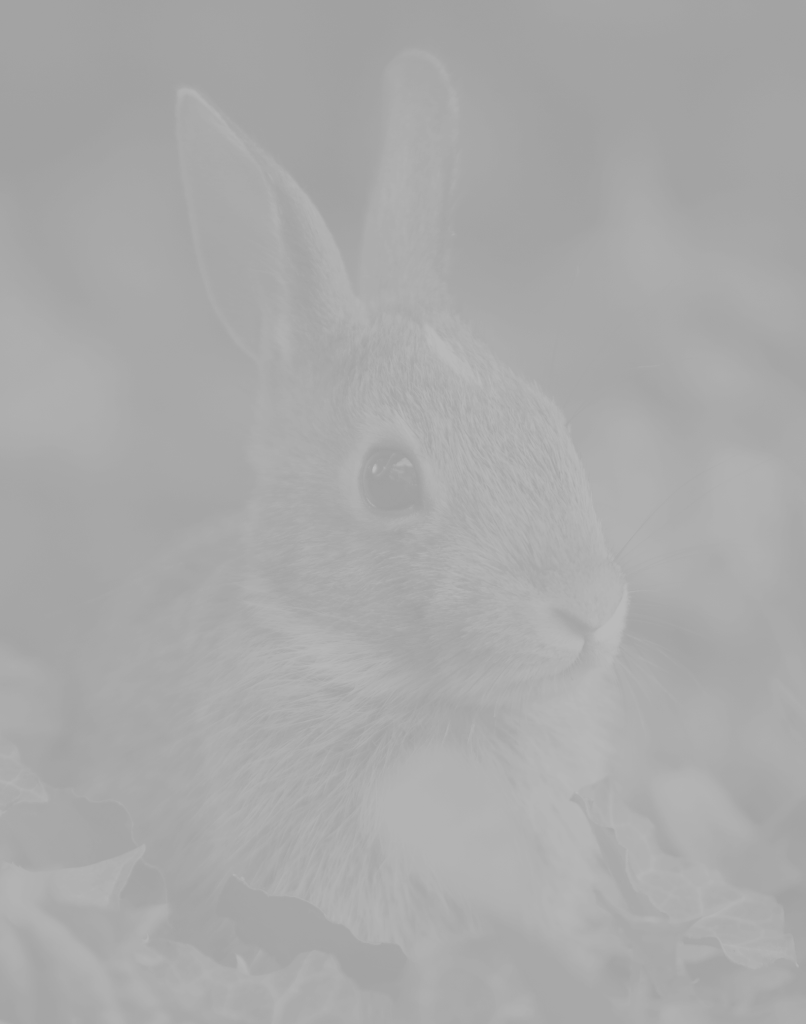
\includegraphics[width=0.7\textwidth]{question3b.png}
    \caption{Question 3b}
    \label{fig:question3b}
\end{figure} \pagebreak
\subsection*{3c}
To improve the image quality, we simply increase the range of the greyscale values. The constants $\alpha$ and $\beta$ can be chosen by determining the transformation that we want to apply to the original histogram. To improve the image quality, we need to increase the contrast of the image by increasing the range of greyscale values. To increase the range of the histogram, we need to multiply all the values by a constant, $\alpha$, which can be determined by dividing our desired range (255) by the range of the original image (28). The adjusted values have to be translated so they start at 0, which is done by changing the value of $\beta$, which must be negative as the values are shifted down towards 0. $\beta$ can be determined by multiplying the minimum greyscale value of the original image (159) and multiplying by $\alpha$. Therefore $\alpha = \sfrac{255}{28}$ and $\beta = -159\cdot(\sfrac{255}{28})$. The Matlab code to perform the transformation is shown in Listing \ref{listing:question3c}.
\lstinputlisting[style=Matlab-editor, caption={Question 3c}, label={listing:question3c},firstnumber=18,firstline=18,lastline=19]{question3.m}
\subsection*{3d}
The MATLAB code to plot and print the final histogram is shown in Listing \ref{listing:question3d}. The final histogram is shown in Figure \ref{fig:question3d}.
\lstinputlisting[style=Matlab-editor, caption={Question 3d}, label={listing:question3d},firstnumber=21,firstline=21,lastline=27]{question3.m}
\begin{figure}[!ht]
    \centering
    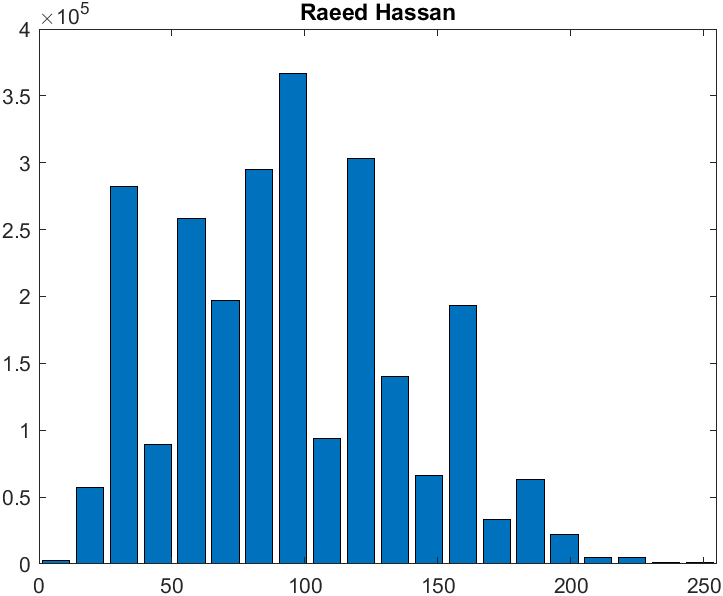
\includegraphics[width=0.8\textwidth]{question3d.png}
    \caption{Question 3d}
    \label{fig:question3d}
\end{figure} \pagebreak
\subsection*{3e}
The MATLAB code to display and print the final image is shown in Listing \ref{listing:question3e}. The final image is shown in Figure \ref{fig:question3e}. The improved image has greater contrast due to the larger range of greyscale values. 
\lstinputlisting[style=Matlab-editor, caption={Question 3e}, label={listing:question3e},firstnumber=29,firstline=29]{question3.m}
\begin{figure}[!ht]
    \centering
    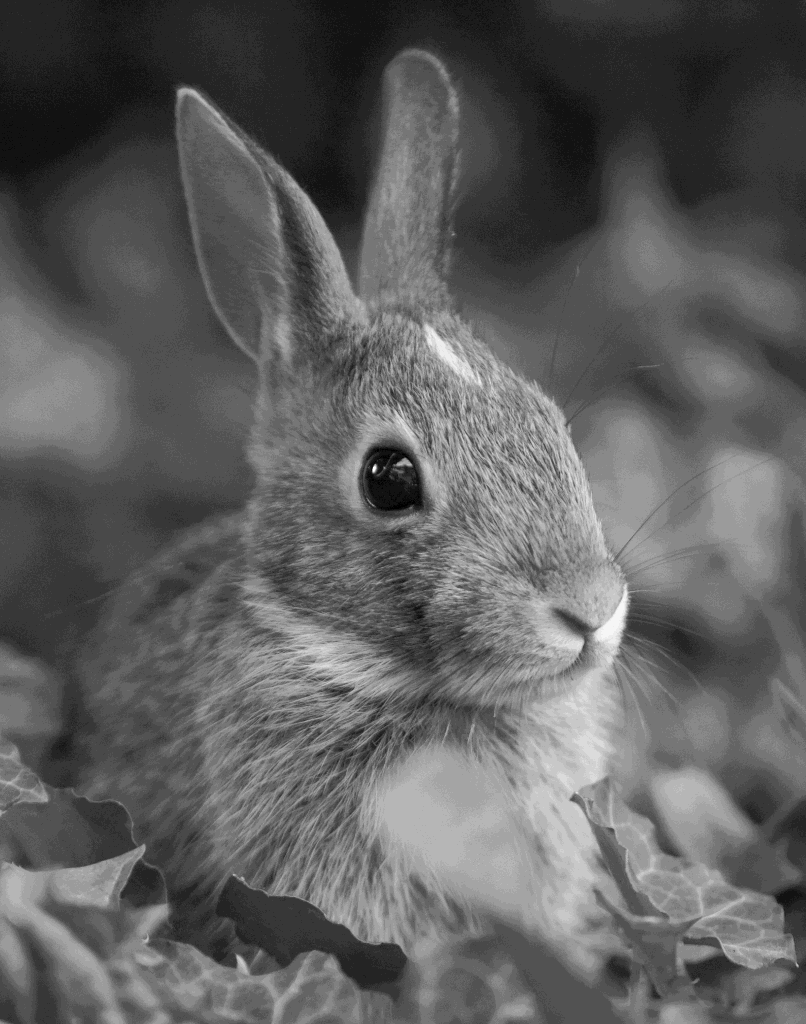
\includegraphics[width=0.8\textwidth]{question3e.png}
    \caption{Question 3e}
    \label{fig:question3e}
\end{figure}
\end{document}